\subsection{点云生成与语义融合模块}
\par 该模块以\texttt{Space}类为主体,使用GPU资源进行实时计算,生成并更新包含RGB信息和语义信息的三维模型。\texttt{Space}类与其他类的关系见图\ref{fig:class4}。模块通过 TSDF 算法生成点云,使用线性分配方法将语义分割信息融入每一个点云中。

\begin{table}[htb]
	\centering
	\caption{Space类的主要成员和方法}
	\label{table:Space}
	\begin{tabular}{|l|m{2.8cm}|m{4.7cm}|m{4.5cm}|}
		\hline
		                     & \multicolumn{1}{c|}{名称}                  & \multicolumn{1}{c|}{类型}                                & \multicolumn{1}{c|}{功能}                         \\ \hline
		\multirow{11}{*}{成员} & \centering\arraybackslash k\_origin\_x   & \centering\arraybackslash const float                  & \centering\arraybackslash \multirow{3}{*}{原点坐标} \\ \cline{2-3}
		                     & \centering\arraybackslash k\_origin\_y   & \centering\arraybackslash const float                  & \centering\arraybackslash                       \\ \cline{2-3}
		                     & \centering\arraybackslash k\_origin\_z   & \centering\arraybackslash const float                  & \centering\arraybackslash                       \\ \cline{2-4}
		                     & \centering\arraybackslash k\_space\_x    & \centering\arraybackslash const float                  & \centering\arraybackslash \multirow{3}{*}{重建范围} \\ \cline{2-3}
		                     & \centering\arraybackslash k\_space\_y    & \centering\arraybackslash const float                  & \centering\arraybackslash                       \\ \cline{2-3}
		                     & \centering\arraybackslash k\_space\_z    & \centering\arraybackslash const float                  & \centering\arraybackslash                       \\ \cline{2-4}
		                     & \centering\arraybackslash k\_point\_size & \centering\arraybackslash const float                  & \centering\arraybackslash 点云分辨率(单位:米)           \\ \cline{2-4}
		                     & \centering\arraybackslash point\_num     & \centering\arraybackslash unsigned int                 & \centering\arraybackslash 点的数量                  \\ \cline{2-4}
		                     & \centering\arraybackslash trunc\_margin  & \centering\arraybackslash float                        & \centering\arraybackslash 截断边界                  \\ \cline{2-4}
		                     & \centering\arraybackslash point\_list    & \centering\arraybackslash Point                        & \centering\arraybackslash 点云结构体数组               \\ \cline{2-4}
		                     & \centering\arraybackslash pcd            & \centering\arraybackslash open3d.geometry.PointCloud   & \centering\arraybackslash Open3D点云对象            \\ \hline
		\multirow{14}{*}{方法} & \centering\arraybackslash InitData       & \centering\arraybackslash void                         & \centering\arraybackslash 点云数据初始化               \\ \cline{2-4}
		                     & \centering\arraybackslash SaveCloud      & \centering\arraybackslash void                         & \centering\arraybackslash 点云模型存储                \\ \cline{2-4}
		                     & \centering\arraybackslash LoadCloud      & \centering\arraybackslash void                         & \centering\arraybackslash 点云模型加载                \\ \cline{2-4}
		                     & \centering\arraybackslash InRange        & \centering\arraybackslash bool                         & \centering\arraybackslash 重建范围判断                \\ \cline{2-4}
		                     & \centering\arraybackslash UpdateScene    & \centering\arraybackslash \_\_global\_\_ void          & \centering\arraybackslash 场景更新                  \\ \cline{2-4}
		                     & \centering\arraybackslash ManageData     & \centering\arraybackslash \_\_host\_\_ void            & \centering\arraybackslash CPU / GPU 数据交换与管理     \\ \cline{2-4}
		                     & \centering\arraybackslash Construct      & \centering\arraybackslash \_\_global\_\_ void          & \centering\arraybackslash 点云生成及语义融合             \\ \cline{2-4}
		                     & \centering\arraybackslash GetNeighbour   & \centering\arraybackslash \_\_device\_\_ vector        & \centering\arraybackslash 获取邻域点的信息              \\ \cline{2-4}
		                     & \centering\arraybackslash DenoiseRGB     & \centering\arraybackslash \_\_device\_\_ void          & \centering\arraybackslash RGB信息滤波               \\ \cline{2-4}
		                     & \centering\arraybackslash DenoiseLabel   & \centering\arraybackslash \_\_device\_\_ void          & \centering\arraybackslash 类别标签滤波                \\ \cline{2-4}
		                     & \centering\arraybackslash ToOpen3DPoint  & \centering\arraybackslash void                         & \centering\arraybackslash Open3D格式转换            \\ \cline{2-4}
		                     & \centering\arraybackslash Downsample     & \centering\arraybackslash void                         & \centering\arraybackslash 八叉树下采样                \\ \cline{2-4}
		                     & \centering\arraybackslash EstimateNormal & \centering\arraybackslash open3d.geometry.PointCloud   & \centering\arraybackslash PCA法线估计               \\ \cline{2-4}
		                     & \centering\arraybackslash GreedyProjTri  & \centering\arraybackslash open3d.geometry.TriangleMesh & \centering\arraybackslash 贪婪投影三角化               \\ \hline
	\end{tabular}
\end{table}

\begin{figure}[htb]
	\centering
	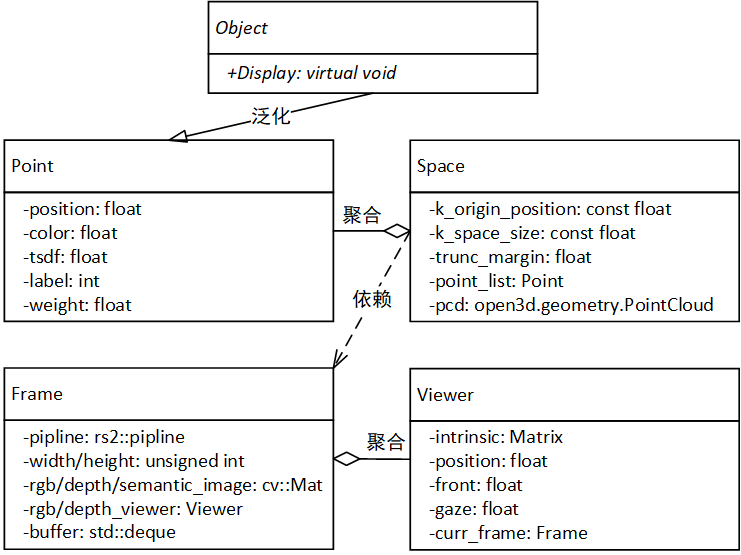
\includegraphics[width=0.7\textwidth]{figures/uml/class4.png}
	\caption{点云生成与语义融合模块类图}
	\label{fig:class4}
\end{figure}

\par 在获取数据预处理与语义分割模块传递来的数据后,通过\texttt{ManageData}函数将CPU中的数据拷贝到GPU内存中。随后,调用\texttt{Construct}进行实时点云的生成,语义融合与更新。\texttt{Construct}输入的参数包括\texttt{Point}类型的点云数组、RGB图像、深度图像、语义分割图像以及内参矩阵和相机位姿。
与\texttt{NormalizeImage}相同,\texttt{Construct}也是一个\texttt{\_\_global\_\_}函数,全部过程运行在GPU上,具体流程如下:

\begin{enumerate}
	\item 根据CUDA线程模型中的\texttt{blockIdx}和\texttt{threadIdx}计算线程序号,并根据这个序号计算当前线程需要处理的点在世界坐标系下的坐标(x, y, z)。

	\item 通过该点的全局三维坐标$P_w$和提供的相机内参、相机位姿,计算出相机坐标$P_{cam}$。根据公式\ref{pose_matrix}可知:
	      \begin{equation}
		      P_{cam} = R^T(P_w - t)
	      \end{equation}

	      因此,可以根据\texttt{pose}计算出该点的相机坐标:
	      \begin{equation}
		      \begin{aligned}
			      x_{cam} = & \texttt{pose[0]} \times (x_w - \texttt{pose[3]}) + \texttt{pose[4]} \times (y_w - \texttt{pose[7]}) \\
			                & + \texttt{pose[8]} \times (z_w - \texttt{pose[11]})                                                 \\
			      y_{cam} = & \texttt{pose[1]} \times (x_w - \texttt{pose[3]}) + \texttt{pose[5]} \times (y_w - \texttt{pose[7]}) \\
			                & + \texttt{pose[9]} \times (z_w - \texttt{pose[11]})                                                 \\
			      z_{cam} = & \texttt{pose[2]} \times (x_w - \texttt{pose[3]}) + \texttt{pose[6]} \times (y_w - \texttt{pose[7]}) \\
			                & + \texttt{pose[10]} \times (z_w - \texttt{pose[11]})
		      \end{aligned}
		      \label{cam_coordinates}
	      \end{equation}

	      计算出相机坐标后,检查该点是否位于相机前方且在预定距离内。如果不在则直接返回,结束当前线程的执行。

	\item 若当前点满足相机视野的条件,则对点进行投影变换,使用相机内参矩阵将其坐标从相机坐标系转换为图像坐标系,即计算出该点在图像中的像素坐标 $P_{pix}$ :
	      \begin{equation}
		      \begin{aligned}
			      x_{pix} = \texttt{intrinsic[0]} \times \frac{x_{cam}}{z_{cam}} + \texttt{intrinsic[2]} \\
			      y_{pix} = \texttt{intrinsic[4]} \times \frac{y_{cam}}{z_{cam}} + \texttt{intrinsic[5]}
		      \end{aligned}
	      \end{equation}

	      然后,判断转换后的像素坐标是否在图像范围内,如果不在则直接返回。

	\item 对于满足以上条件的点,计算其在RGB图像、深度图像和语义分割图像中的位置,并读取对应位置的RGB值、深度值和类别标签,对深度值进行检查,如果值过小或过大,则直接返回。

	\item 点云生成,计算点的TSDF值。TSDF值即点相对于观测到的表面的距离,通过该点在相机视野中的深度和真实深度之间的差值来计算。如果计算得到的TSDF值小于截断范围的负值,则直接返回。否则,在1.0f和自身与截断范围的比值之间取较小值,使用一个权重系统与旧的TSDF值进行加权平均更新TSDF值,以处理多个视角的影响,公式如下:
	      \begin{equation}
		      TSDF_{i} = \frac{TSDF_{i-1} \times W_{i-1} + tsdf_{i} \times w_{i}}{W_{i-1} + w_{i}}
	      \end{equation}

	      \par 这里的 $TSDF_{i-1}$ 和 $W_{i-1}$ 即当前点存储的前 $i-1$ 次更新的 TSDF 值和权重,$tsdf_{i}$ 是根据当前深度图计算出来的第$i$帧的 TSDF 值,$w_{i}$ 是当前更新的权重。

	\item 实时语义融合与更新。这里采取与 Panopticfusion相似的方法,在每次将某个点匹配到目标类别标签以及置信度后,使用线性分配的方式更新类别标签\cite{panopticfusion,VolumetricMethod},具体方法如下:

	      \par 对于每个时间步长$t$和体素$v$,根据公式
	      \begin{equation}
		      W(t, v)=\left\{\begin{array}{ll}
			      W(t-1, v)+w(t, v) & l_{d}(t, v)=l_{\tau}(t, v)                                    \\
			      W(t-1, v)-w(t, v) & l_{d}(t, v) \neq l_{\tau}(t, v) \wedge W(t-1, v) \geq w(t, v) \\
			      w_{t}(v, d)       & l_{d}(t, v) \neq l_{\tau}(t, v) \wedge W(t-1, v)<w(t, v)
		      \end{array}\right.
		      \label{equ:lap}
	      \end{equation}

	      计算权重 $W(t, v)$,其中 $l_{\tau}(t, v) \in L$ 和 $w(t, v)$ 是当前点在前图像帧中关联的目标类别标签的全局序号和置信度,$l_{d}(t, v) \in L$ 和 $W(t-1, v)$ 是当前点在先前图像帧中已经关联的目标类别标签的全局序号和置信度,即\texttt{label}和\texttt{label\_weight}。
	      如果在当前图像帧中该点的置信度显著减小,例如当 $l_{d}(t, v) \neq l_{\tau}(t, v) \land W(t - 1, v) < w(t, v)$ 时,会重置该点的全局序号为 $l_{d}(t, v)$,如公式\ref{equ:lap}中的最后一种情况所示。这样,每个点只需要存储一个类别标签的全局序号,而不需要记录每个点关联的所有类别标签。

	      \begin{algorithm}[htbp]
		      \SetAlgoLined
		      \KwData{点云结构体数组 point\_list, RGB图像 rgb\_image, 深度图像 depth\_image, 语义分割图像 semantic\_image, 相机内参 intrinsic, 相机位姿(外参) pose}
		      \KwResult{更新后的包含语义信息的点云}
		      \ForEach{thread in GPU}{
			      使用blockIdx和threadIdx计算线程索引\;
			      根据线程索引从 $point_list$ 获取当前点 $p$\;
			      根据 $intrinsic$、$intrinsic$ 计算当前点的相机系坐标\;
			      \If{$p$ 不在相机前方或不在预设距离内}{
				      继续\;
			      }
			      使用 $intrinsic$ 将 $p$ 的相机系坐标 $p_{c}$ 转换为图像系坐标 $p_{i}$\;
			      \If{$p_{i}$ 不在图像范围内}{
				      继续\;
			      }
			      将 $p$ 投影到 $rgb\_image$、$depth\_image$ 和 $semantic\_image$\;
			      获取 $p$ 相应的RGB值、深度值和类别标签\;
			      \If{深度值不在合理范围内}{
				      继续\;
			      }
			      为 $p$ 计算TSDF值\;
			      \If{TSDF值小于截断范围的负值}{
				      继续\;
			      }
			      使用加权平均方法更新TSDF值\;
			      使用线性分配方法更新类别标签\;
		      }
		      \caption{Construct}
		      \label{algo:ConstructAlgorithm}
	      \end{algorithm}

	      由于在全景分割中很难定义类别标签的权重\cite{EfficientPS},所以假权重对于所有检测到的类别为1,对于其他类别为0。根据公式

	      \begin{equation}
		      class(t, l)=\left\{
		      \begin{array}{ll}
			      argmax_c(n_c^l/n^l) & max_c(n_c^l/n^l) \geq \theta \\
			      null                & max_c(n_c^l/n^l) \leq \theta
		      \end{array}\right.
	      \end{equation}

	      确定该点在进行第 $t$ 次语义融合时的类别标签 $l \in L$。其中,$n_l^c$ 是该点与类别 $c$ 关联的次数,而 $n^{l}$ 是该点在所有类别中的关联
	      总次数。如果得分低于给定的阈值 $\theta$,类别标签将被分配到 $null$ 类,代表该语义分割算法无法识别此对象。

\end{enumerate}

\par \texttt{Construct}函数的伪代码如算法\ref{algo:ConstructAlgorithm}所示。

\par 经过上述步骤后,就可得到一个包含RGB信息和语义信息的三维点云模型。模型中每个类别的精度可以使用交并比(Intersection Over Union,IoU)衡量,伪代码如算法\ref{algo:EvaluateSemanticSegmentation}所示。

\begin{algorithm}[htbp]
	\SetAlgoLined
	\KwData{场景序号 scene\_id, 预测模型路径 pred\_model\_path, GT模型路径 gt\_model\_path}
	\KwResult{IoU 列表}
	初始化类别标签的映射字典 $category\_id$\;
	读取预测模型数据 $pred\_model$,并将尺寸放大 20 倍\;
	初始化点云查找表 $point\_cloud\_table$\;
	将预测模型中的每个点的标签存储在 $point\_cloud\_table$ 相应的空间位置上\;
	读取 Ground Truth 模型数据 $gt\_model$,并与预测模型进行坐标对齐\;
	初始化预测模型的类别标签数组 $pred\_count[category\_id.size()]$\;
	初始化GT模型的类别标签数组 $gt\_count[category\_id.size()]$\;
	初始化整数数组 $intersect\_count[category\_id.size()]$用于表示预测点和GT点一致\;
	\For{$point$ in $gt\_model$}{
		\If{point in $point\_cloud\_table$}{
			$gt\_count[point.label]++$\;
			$pred\_count[point\_cloud\_table.get(point).label]++$\;
			\If{point.label == $point\_cloud\_table.get(point).label$}{
				$intersect\_count[point.label]++$\;
			}
		}
	}
	初始化列表 $IoU[category\_id.size()]$记录每个类别标签的IoU值\;
	\For{$i$ in $0$ to $category\_id.size()$}{
		$IoU[i] = intersect\_count[i] / (pred\_count[i] + gt\_count[i] - intersect\_count[i])$\;
	}
	% 将 $IoU$ 值保存在 CSV 文件 $iou\_results.csv$ 中\;
	\caption{EvaluateSegmentation}
	\label{algo:EvaluateSemanticSegmentation}
\end{algorithm}